\documentclass[conference]{IEEEtran}
\IEEEoverridecommandlockouts
% The preceding line is only needed to identify funding in the first footnote. If that is unneeded, please comment it out.
\usepackage{cite}
\usepackage{amsmath,amssymb,amsfonts}
\usepackage{algorithmic}
\usepackage{graphicx}
\usepackage{textcomp}
\usepackage{xcolor}
\def\BibTeX{{\rm B\kern-.05em{\sc i\kern-.025em b}\kern-.08em
    T\kern-.1667em\lower.7ex\hbox{E}\kern-.125emX}}
\begin{document}

\title{CYBER RISK AND CYBER INSURANCE\\}

\author{\IEEEauthorblockN{Suraj Eswaran}
\IEEEauthorblockA{\textit{Colorado State University} \\
\textit{Fort Collins,Colorado}\\
suraj22@colostate.edu}
\and
\IEEEauthorblockN{Prof. Yashwant K. Malaiya}
\IEEEauthorblockA{\textit{Colorado State University} \\
\textit{Fort Collins,Colorado}\\
malaiya@cs.colostate.edu}
}


\maketitle

\begin{abstract}
Cyber risk is a form of risk from the exposure resulting from a cyber-attack or data breach. Organizations tend to become more vulnerable to these kinds of threats due to their high reliability on computers, networks, and information in order to get along with the delivery of the services. In case of failure in these systems, these organization will face a negative impact in the processes , which will create a negative impact on the organization. So, this paper deals with the understanding the various views on cyber risk insurance and its challenges that arises in insurance markets in the recent years.   
\end{abstract}

\begin{IEEEkeywords}
Cyber risk, Cyber risk Insurance, Risk avoidance,insurance premium,Cyber security.
\end{IEEEkeywords}
\section{Introduction}

\section{Discussion Of Background Literature}
\subsection{Analysis and Modelling of Cyber Risk}
    According to Inversion Model Expert System, there has been a shift from manual to automation which tend to change from external risk to internal risks. The external threats are related to process whereas internal threats with information. From this, several aspects has been proposed in creating models with various scenarios. Kokolakis et.al\cite{b1} have utilized IT risk with the help of BPM(Business Process Modeling) which is a method of controlling the process in a phase of crisis. This approach relies on the mixture of risk analysis with business procedure , thus support Information Security Analysis and Design. Pernul et al.\cite{b2} have focused on developing a secured business process based on security requirements. 
    \\Similar work was proposed by Roehrig et al.\cite{b3} and Ribeiro et al.\cite{b4} where they proposed it against security policies. Halliday et al.\cite{b5}  conducted risk analysis with high level  business strategy. Whereas Rodriguez et. al.\cite{b6} elaborated the analysis of Business Process Modelling Notation with security requirements. Furthermore, there were few more analysis where they have also utilized Business Process Model, like Suh and Han\cite{b7} and Rainer et al.\cite{b8} where they have proposed at various scenarios. 
    \subsection{Controlling the risk using Cyber Insurance}
    Cyber Insurance depends on the organization’s exposure to cyber risk and data breaches. The market for insuring against these has been  grown rapidly in the past decade. Cyber insurance has been the term utilizes first and third-party losses that results in loss due to system-based attack. Several approaches have provided an excellent elaboration of cyber insurance. Böhme and Schwartz\cite{b9} defined a unified model for cyber insurance with some structural details of the business protocol.In addition to theoretical model, Marotta et al.\cite{b10}compared various approaches of cyber insurance market and direction towards further advances in cyber insurance. Majuca et. al.\cite{b11} describes evolution of cyber insurance in 2005 which focusses on analysis of market with discussion of several problems. Woods et al.\cite{b12} determines insurance carriers by examining 14 questionnaires. 
    \\Romanosky et al. examined  over recent top 100 cyber insurance policies with state insurance policies\cite{b13}. It is very difficult to find businesses without cyber insurance pricing in order to store sensitive information. Cyber Criminals will target large organization so that they can take away more money with lot of damages. Thus, it is necessary to focus on the pricing aspect of cyber insurance. Mukhopadhyay et. al.\cite{b14} developed Utility Based Preferential Pricing(UBPP) in order to help the organization, decide on the pricing aspect of cyber insurance products. Similarly, Hemantha and Tejaswini\cite{b15} utilized a scheme called Copula-based cyber-insurance model (CBCI) where they fitted a copula to the empirical values and computed the expected value. But, Ulrik Franke\cite{b16} documented the empirical study pf cyber insurance market in Sweden with 10 different insurance companies and provided an analysis for average pricing of cyber insurance. 

\section{Summary of the Investigations/Findings}

Recent studies have only focused on the market analysis and discussion of cyber risk. But they fail to provide a survey of various aspects of cyber risk and cyber insurance. Thus, this paper discusses on various approaches from various researchers from market and scientific perspective. We have examined practical techniques with a mathematical model for the future scope of scientific perspective in the field of cyber insurance. 

Based on the existing studies, there are five main factors for developing cyber risk management. In order to maintain an efficient and relative cyber risk management, it is necessary to have a proper evaluation and risk control.  
\begin{figure}
\centering
  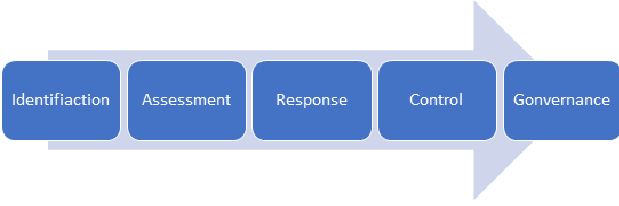
\includegraphics[width=0.9\columnwidth]{fig1.png}
  \caption{Factors involving Risk Management}~\label{fig:figure1}
\end{figure}

\begin{itemize}
    \item Risk Identification: Identification shows the vulnerabilities due to cyber risk which causes the consequences for assets due to breaches. With regards to this, the organization need to find out risk control measures. For that, they utilize either top-down or bottom-up technique. Top-down points out the main threats from the strategic point of view whereas bottom-up tends to be featuring detailed evaluation of threats. It is advisable to utilize bottom-up technique as top-down might not identify few risks which creates correlation. Risk identification  is conducted with the help of questionnaires regarding business activities or network security. In the case of complex risks, insurance companies utilize technical handwriting.  
\item Risk Assessment: The organization need to expose the risk and check whether it can be assessed or not which includes estimation of loss due to cyber risk and assessment of risk level. Along with that, the amount of long-term profit loss share will be calculated which share the majority of share in cyber risk loss. 
\item Risk Response:Response involves three methods to measure the response of the risk. They are avoidance, mitigation, and acceptance, which shows amount loss from the incident.

\begin{itemize}
\item Avoidance: It involves elimination of activities and exposures which affects the organization.
\item Mitigation: A strategy which is utilized for reducing the adverse effects due to the cyber risks. 
\item Acceptance: It is a process of choosing the option depending on the user agreed level of appropriate cyber risk.
\end{itemize}
\item Control: After the identification, evaluation and processing of cyber risk , the next step would be controlling of risk. Organization need to regularly monitor their risk and improve these factors. 
\item Governance: Governance is needed in order to finish a complete cyber risk risk management. It focusses on organization’s culture and develops awareness within all the employees, thus provides instructions on IT security. 
\\
\\With higher sensitive information and information system, the implementation of organization based cyber risk management with proper response level is necessary. From the above discussion we can infer that proper IT security requirements as well as insurance policy coverage can lower the risk exposure or even loss. Organization that depend on Internet services or cloud services should look over their risk positions, in the case of crashes of website, there will be a drop in the incomes which tend to allow customers to go for different products. There will be reduction in the market value if the situation of log term cyber risk occurrence. Thus, it is necessary for an organization to get along with cyber risk management with assessment, evaluation, and improvement. Risk awareness has to be helpful in providing a good risk management system for the organization.

\begin{figure}
\centering
  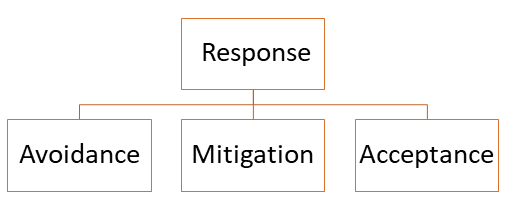
\includegraphics[width=0.9\columnwidth]{fig2.png}
  \caption{Characteristics of Response}~\label{fig:figure2}
\end{figure}
\begin{itemize}

\item Cyber risk has been serious issue with increase in virtual interactions during the pandemic. Due to this, there has been an increase in surface for the attacker which doubted the organization’s integrity, confidentiality, and availability factors in year 2020. From various sources we can infer various facets of cyber risk. 
\item According to Gartner Research, there will be an increase of global information security market in the year 2022, to a range of 170.4 billion dollars\cite{b17}.
\item According to Symantec, one out of 36 mobile devices tend to have high risk application and one out of 13 web request causes malware\cite{b18}.
\item	Average cost of cyber crime tend to be 14.7 million dollars which is 68 more than what we obtained in the year 2019\cite{b19}. 
\item	Cyber risk of 2020 includes new and insecure usage of software because after the transaction from office to home there has been a high usage of new software in order to reduce the distance between the customer and consumers. But it does not guarantee that these software are secure enough and implementation of these software. 
\item Beginning of the corona pandemic, cyber criminals utilized this situation, and it has been reported that there were thousands of scams and malicious websites created every day which results in phishing of data.  
\item Processing of these sensitive data would be one of the biggest risks in 2020. 
\end{itemize}
\end{itemize}
\section{Any Refinements of the Proposal Objectives as a Result of the Past Study}
For this paper, we have utilized the framework by Bohme and Schewartz which features properties of cyber risk in a unified manner. The framework implements all the modelling papers that deals with cyber insurance with terminology. This brings us to compare between different models in order to get a view on decisions with what kind of outcomes.
The components implemented in this framework: 

\begin{figure}
\centering
  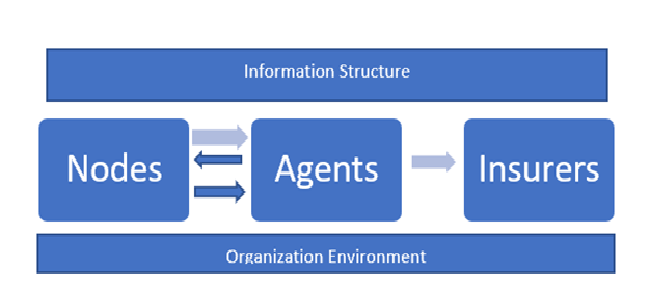
\includegraphics[width=0.9\columnwidth]{fig3.png}
  \caption{Implemented Model for Cyber Insurance Market}~\label{fig:figure2}
\end{figure}



\begin{itemize}
\item Agents: Entities which are on the demand part of the cyber insurance model. They are responsible for controlling the nodes. It has several features like node control, space, time, heterogeneous, and aversion. Node control explains the mapping between agents where each node can only be possible to be controlled by single agent. Aversion happens when there is a dispersion in income distribution with its expected value. Different models tend to product action space with respect to insurance premium. Thus, it is required to maintain time, heterogeneous and space. 
\item Nodes: Nodes are controlled by agents which are atomic level of the network. Risk arrival method is also called as per-node process.   
\item Insurers: Entities which are on the supply side of the cyber insurance model. It has several features like market structure, aversion, markup, design, and risk transfer. Market structure involves the number of insurers: monopoly, oligopoly, and competition. Aversion happens when there is a dispersion in income distribution with its expected value. Design provides a definition for agent’s space where it can provide as a set of tuples. 
\end{itemize}

The study explores the different views of cyber risk that has emerged in the recent years. First approach deals with the study of Operational Risk which is risk that are caused by the actual losses due to inappropriate procedures, systems or policies followed by the organizations\cite{b20} \cite{b21}. It focuses on how things are accomplished in an organization and not on what is produced from that organization. So, operational risk can be utilized as a technique to get along with this exposure.

Second approach deals with utilization of a mechanism for avoiding cyber risk that seeks to remove the possibility of activities that creates risk\cite{b14}. Cyber risk insurance is a tool that are useful to compensate the loss from the cyber risk incidents\cite{b14}\cite{b22}. For this study, we are preparing the various components for an efficient cyber risk management by analyzing internal risk management with risk awareness factors.  



Transaction from traditional business models to modern models made it create more vulnerability as more of digitalization made the chance for cyber risk. Furthermore, it is necessary to have intangible assets for determining threats and losses. Insufficient data can also be a treat as it would be difficult in situations of cyber risk incidents as information is needed to report a risk. 

\begin{thebibliography}{00}
\bibitem{b1} S. Kokolakis, A. Demopoulos and E. Kiountouzis, “The use of business process modeling in information systems security analysis and design,” Inf.Manag. and Comp. Security, 8, 2000, p. 107-116.
\bibitem{b2}Herrmann, G., & Pernul, G. (1998, January). Towards security semantics in workflow management. In Proceedings of the Thirty-First Hawaii International Conference on System Sciences (Vol. 7, pp. 766-767). IEEE.
\bibitem{b3}S. Roehrig and K. Knorr, “Security Analysis of Electronic Business Processes,” Electronic Commerce Research, vol. 4, 2004, P. 59-81.
\bibitem{b4} C. Ribeiro and P. Guedes, “Verifying Workflow Processes against Organization Security Policies,” 8th IEEE International Workshops on Enabling Technologies, 1999, P. 190-191.
\bibitem{b5}S. Halliday, K. Badenhorst and R. von Solms, “A business approach to effective information technology risk analysis and management“ Information Management&Computer Security, vol. 4/1, 1996, P. 19–31.
\bibitem{b6} A. Rodriguez, E. Fernandez-Medina and M. Piattini, “A BPMN Extension for the Modeling of Security Requirements in Business Processes,” IEICE Trans. INF. & SYST., vol. E90–D, Apr. 2007.  
\bibitem{b7} B. Suh und I. Han, “The IS risk analysis based on a business model,” Information & Management, vol. 41, 2003, P. 149–158.
\bibitem{b8} R.K. Rainer, C.A. Snyder and H.H. Carr, “Risk Analysis for Information Technology,” Journal of Management Information Systems, vol. 8, 1991, P. 129-147.
\bibitem{b9} Böhme R, Schwartz G. Modeling cyber-insurance: towards a unifying framework. In: Workshop on the Economics of Information Security (WEIS). Cambridge, MA: Harvard University, 2010.
\bibitem{b10} Marotta, A., Martinelli, F., Nanni, S., & Yautsiukhin, A. (2015). A survey on cyber-insurance. Technical Rep. IIT TR-17/2015. Istituto di Informatica e Telematica, Consiglio Nazionale delle Richerce, Pisa.
\bibitem{b11} Majuca, R. P., Yurcik, W., & Kesan, J. P. (2006). The evolution of cyberinsurance. arXiv preprint cs/0601020. 
\bibitem{b12} Woods, D., Agrafiotis, I., Nurse, J. R., & Creese, S. (2017). Mapping the coverage of security controls in cyber insurance proposal forms. Journal of Internet Services and Applications, 8(1), 8.
\bibitem{b13} Romanosky, S., Ablon, L., Kuehn, A., & Jones, T. (2017). Content analysis of cyber insurance policies: How do carriers write policies and price cyber risk?. Available at SSRN 2929137.
\bibitem{b14} Mukhopadhyay, A., Chatterjee, S., Saha, D., Mahanti, A., & Sadhukhan, S. K. (2013). Cyber-risk decision models: To insure IT or not?. Decision Support Systems, 56, 11-26.
\bibitem{b15} Herath, H., & Herath, T. (2011). Copula-based actuarial model for pricing cyber-insurance policies. Insurance markets and companies: analyses and actuarial computations, 2(1), 7-20.
\bibitem{b16} Franke, U. (2017). The cyber insurance market in Sweden. Computers & Security, 68, 130-144.
\bibitem{b17} Gartner Inc. (n.d.). Forecast Analysis: Information Security, Worldwide, 2Q18 Update. Retrieved November 08, 2020, from https://www.gartner.com/en/documents/3889055
\bibitem{b18} Symantec Security Center. (n.d.). Retrieved November 08, 2020, from https://www.broadcom.com/support/security-center
\bibitem{b19} Böhme, R., & Schwartz, G. (2010, June). Modeling Cyber-Insurance: Towards a Unifying Framework. In WEIS.
\bibitem{b20} Romanosky, S., Ablon, L., Kuehn, A., & Jones, T. (2019). Content analysis of cyber insurance policies: how do carriers price cyber risk?. Journal of Cybersecurity, 5(1), tyz002.
\bibitem{b21} Falco, G., Eling, M., Jablanski, D., Miller, V., Gordon, L. A., Wang, S. S., ... & Donavan, E. (2019). A research agenda for cyber risk and cyber insurance. In Workshop on the Economics of Information Security (WEIS)..
\bibitem{b23} Camillo, M. (2017). Cyber risk and the changing role of insurance. Journal of Cyber Policy, 2(1), 53-63.

\end{thebibliography}

\end{document}
